\chapter{झिल्लियाँ और झिल्ली-अभिगमन}\label{ch:b1:membranes-transport}

किसी लाल रक्त \omterm{def:b1:cell-unit-of-life:cell}{कोशिका} को शुद्ध जल में डालिए और वह सेकंड भर में फूलकर फट
जाती है; उसे गाढ़े नमक में डालिए और वह सिकुड़ जाती है। उसे वापस
प्लाज़्मा में रखिए और वह चार महीने अपना उभयावतल रूप बनाए रखती है, और उस
पूरे समय हर सेकंड सोडियम बाहर तथा पोटैशियम भीतर पंप करती रहती है। जो
झिल्ली यह करती है वह पाँच नैनोमीटर मोटी है --- दो अणु गहरी लिपिड की एक
झिल्ली, जिसमें प्रोटीन पिरोए हैं --- और वही वह सीमा है जिसके आरपार
\cref{ch:b1:organism-environment} का हर विनिमय अंततः होता है। यह अध्याय
झिल्ली की संरचना, बिना सहायता उसे पार करने वाली चीज़ों की भौतिकी, बाक़ी
को ढोने, पंप करने और \omterm{def:b1:membranes-transport:transporters}{चैनल} से निकालने वाले प्रोटीनों, इस आवागमन से बनते
विद्युत विभव, और उन पुटिकाओं का वर्णन करता है जो वह ढोती हैं जिसे कोई
प्रोटीन नहीं ढो सकता।

\section{तरल मोज़ेक}

\begin{definition}[प्लाज़्मा झिल्ली]\label{def:b1:membranes-transport:membrane}
\emph{प्लाज़्मा झिल्ली}\index{प्लाज़्मा झिल्ली} --- और \omterm{def:b1:cell-unit-of-life:cell}{कोशिका} की हर
झिल्ली --- लगभग \qty{5}{nm} मोटा एक \emph{लिपिड
द्विस्तर}\index{लिपिड द्विस्तर} है: फ़ॉस्फ़ोलिपिडों की दो चादरें
(\cref{ch:b1:lipids}), जिनकी जलविरागी पूँछें एक-दूसरे की ओर हैं और
ध्रुवीय सिर दोनों जलीय ओर, पूँछों के बीच कोलेस्टेरॉल, और उसमें धँसे या
उससे लगे \emph{झिल्ली प्रोटीन}\index{झिल्ली प्रोटीन}। \emph{तरल
मोज़ेक}\index{तरल मोज़ेक मॉडल} मॉडल (सिंगर और निकोल्सन, 1972) में
द्विस्तर एक द्विविमीय तरल है जिसमें लिपिड और प्रोटीन पार्श्व दिशा में
विसरित होते हैं, और प्रोटीन स्वतंत्र इकाइयों का एक मोज़ेक हैं, कोई सतत
लेप नहीं। दोनों फलक भिन्न हैं: लिपिडों और प्रोटीनों से जुड़ी शर्कराएँ
केवल बाहर की ओर होती हैं (\emph{ग्लाइकोकैलिक्स}), और कुछ फ़ॉस्फ़ोलिपिड
केवल एक ही पर्ण तक सीमित रहते हैं।
\end{definition}

\begin{omfigure}
\begin{tikzpicture}[font=\footnotesize, line cap=round]
  % bilayer: heads as circles, tails as lines
  \foreach \i in {0,...,21} {
    \pgfmathsetmacro{\x}{0.42*\i}
    \fill[omDef!60] (\x,1.35) circle (0.16);
    \draw[omDef!70!black, thick] (\x-0.07,1.2) -- (\x-0.07,0.55) (\x+0.07,1.2) -- (\x+0.07,0.55);
    \fill[omDef!60] (\x,-0.35) circle (0.16);
    \draw[omDef!70!black, thick] (\x-0.07,-0.2) -- (\x-0.07,0.45) (\x+0.07,-0.2) -- (\x+0.07,0.45);
  }
  % cholesterol
  \foreach \x in {1.9,6.1,8.2} { \draw[omProp, very thick] (\x,1.1) -- (\x,0.6); \fill[omProp] (\x,1.15) circle (0.08); }
  % integral protein spanning (channel)
  \draw[thick, omThm!80!black, fill=omThm!30, rounded corners=3pt] (3.0,-0.7) rectangle (3.55,1.7);
  \draw[thick, omThm!80!black, fill=omThm!30, rounded corners=3pt] (3.85,-0.7) rectangle (4.4,1.7);
  \fill[white] (3.55,-0.6) rectangle (3.85,1.6);
  % integral protein (carrier)
  \draw[thick, omThm!80!black, fill=omThm!30, rounded corners=5pt] (6.8,-0.75) rectangle (7.7,1.75);
  % peripheral protein
  \draw[thick, omExo!80!black, fill=omExo!30] (5.3,1.75) ellipse (0.5 and 0.28);
  % glycocalyx sugar chains on outer face
  \foreach \x in {0.5,1.3,2.5,4.15,7.25,8.4} { \draw[omProp!80!black, thick] (\x,1.5) .. controls (\x+0.15,1.85) and (\x-0.15,2.1) .. (\x+0.1,2.4); \fill[omProp!70] (\x+0.1,2.45) circle (0.07); }
  % labels
  \node[anchor=east] at (-0.3,1.35) {ध्रुवीय सिर};
  \node[anchor=east] at (-0.3,0.5) {जलविरागी पूँछें};
  \node[anchor=east] at (-0.3,-0.35) {ध्रुवीय सिर};
  \node[anchor=west, align=left] at (9.2,2.2) {शर्करा-शृंखलाएँ: केवल बाहर};
  \node[anchor=west, align=left] at (9.2,0.5) {\qty{5}{nm}};
  \node[anchor=north] at (3.7,-0.95) {चैनल प्रोटीन};
  \node[anchor=north] at (7.25,-0.95) {वाहक प्रोटीन};
  \node[anchor=south] at (5.3,2.6) {परिधीय प्रोटीन};
  \node[anchor=north, omProp] at (1.5,-1.0) {कोलेस्टेरॉल};
  \node[anchor=south east, gray] at (-0.3,2.4) {बाहर};
  \node[anchor=north east, gray] at (-0.3,-0.95) {कोशिकाद्रव};
  \draw[<->, gray] (9.05,1.35+0.16) -- (9.05,-0.35-0.16);
\end{tikzpicture}

{\small \omterm{def:b1:membranes-transport:membrane}{तरल मोज़ेक}। फ़ॉस्फ़ोलिपिडों के दो पर्ण, पूँछें भीतर की ओर,
उनके बीच कोलेस्टेरॉल; द्विस्तर को पार करते \omterm{def:b1:membranes-transport:proteins}{अंतर्वेशी प्रोटीन} (छिद्र सहित
एक \omterm{def:b1:membranes-transport:transporters}{चैनल}, एक वाहक), एक फलक पर एक परिधीय प्रोटीन, और शर्करा-शृंखलाएँ केवल
बाहरी फलक पर।}
\end{omfigure}

\begin{omfigure}
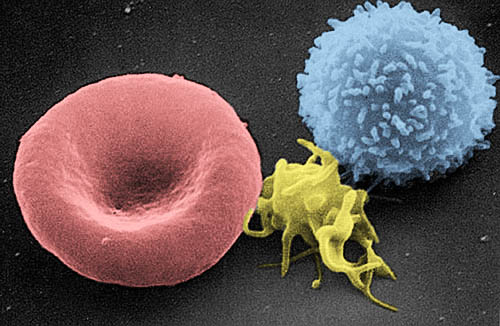
\includegraphics[width=0.4\linewidth]{images/book3/red-cells-nci.jpg}

{\small क्रमवीक्षण \omterm{prop:b1:cell-unit-of-life:microscopes}{इलेक्ट्रॉन सूक्ष्मदर्शी} के नीचे एक लाल रक्त \omterm{def:b1:cell-unit-of-life:cell}{कोशिका},
एक बिंबाणु और एक लसीकाणु (रंग चढ़ाकर)। लाल \omterm{def:b1:cell-unit-of-life:cell}{कोशिका} का उभयावतल रूप उसकी
झिल्ली के नीचे के प्रोटीन जाल से थमा है; वह अपने से भी सँकरी केशिकाओं से
दबकर निकलते हुए चार महीने बिता देती है। चित्र: राष्ट्रीय कैंसर संस्थान,
सार्वजनिक अधिकार-मुक्त।}
\end{omfigure}

\begin{proposition}[झिल्लियाँ द्विस्तर हैं और तरल हैं]\label{prop:b1:membranes-transport:evidence}
\omterm{def:b1:membranes-transport:membrane}{प्लाज़्मा झिल्ली} ठीक दो लिपिड अणु मोटी है, और उसके घटक उसके तल के भीतर
चलते हैं।
\end{proposition}
\begin{proof}[साक्ष्य]
गॉर्टर और ग्रेंडल (1925) ने ज्ञात संख्या की लाल रक्त \omterm{def:b1:cell-unit-of-life:cell}{कोशिकाओं} के लिपिड
निकाले और उन्हें जल पर एकल परत के रूप में फैलाया: क्षेत्रफल \omterm{def:b1:cell-unit-of-life:cell}{कोशिकाओं} की
कुल सतह से दुगुना निकला, इसलिए झिल्ली एक द्विस्तर है। इलेक्ट्रॉन
सूक्ष्मदर्शिकी हर झिल्ली को किसी फीके अंतर्भाग (पूँछें) के चारों ओर दो
गहरी रेखाओं (रंगे हुए सिर) के रूप में दिखाती है, कुल मिलाकर
\qty{5}{nm}। फ़्राई और एडिडिन (1970) ने एक मूषक \omterm{def:b1:cell-unit-of-life:cell}{कोशिका} को एक मानव
\omterm{def:b1:cell-unit-of-life:cell}{कोशिका} से जोड़ा जिसके सतही प्रोटीन दो रंगों के रंजकों से चिह्नित थे:
\qty{37}{\celsius} पर चालीस मिनट बाद दोनों रंग संकर \omterm{def:b1:cell-unit-of-life:cell}{कोशिका} पर पूरी तरह
मिल चुके थे, और \qty{4}{\celsius} पर नहीं, जहाँ लिपिड लगभग ठोस है।
किसी प्रतिदीप्त \omterm{def:b1:membranes-transport:membrane}{झिल्ली प्रोटीन} के एक धब्बे को लेज़र से विरंजित करके और
अविरंजित अणुओं के विसरित होकर भीतर आते जाने पर प्रतिदीप्ति लौटते देखना
(FRAP) पार्श्व विसरण मापता है: लिपिडों के लिए कुछ सेकंड में
$\qty{1}{\micro m^2}$, प्रोटीनों के लिए धीमा, और \omterm{def:b1:eukaryotic-cell:cytoskeleton}{कोशिका-कंकाल} से बँधे
प्रोटीनों के लिए शून्य।
\end{proof}

\begin{definition}[झिल्ली प्रोटीन]\label{def:b1:membranes-transport:proteins}
\emph{अंतर्वेशी}\index{अंतर्वेशी प्रोटीन} \omterm{def:b1:membranes-transport:membrane}{झिल्ली प्रोटीन} एक या अधिक
जलविरागी कुंडलियों से द्विस्तर को पार करते हैं और केवल अपमार्जकों से ही
निकाले जा सकते हैं; \emph{परिधीय} प्रोटीन किसी एक फलक से बँधे होते हैं।
कार्य के अनुसार: \emph{अभिगमक} (\omterm{def:b1:membranes-transport:transporters}{चैनल}, वाहक, पंप), \emph{ग्राही} जो बाहर
किसी संकेत से बँधते हैं और भीतर क्रिया करते हैं, \emph{एंजाइम},
\emph{लंगर} जो \omterm{def:b1:eukaryotic-cell:cytoskeleton}{कोशिका-कंकाल} को \omterm{def:b1:body-plans-tissues:connective}{बाह्यकोशिकीय आधात्री} से जोड़ते हैं, और
\emph{अभिज्ञान} प्रोटीन जो वे शर्कराएँ धारण करते हैं जिनसे \omterm{def:b1:cell-unit-of-life:cell}{कोशिकाएँ}
एक-दूसरे को पहचानती हैं। प्रोटीन किसी प्रारूपिक झिल्ली के द्रव्यमान का
आधा हैं और उसके कार्य के लगभग पूरे।
\end{definition}

\section{बिना सहायता झिल्ली पार करना}

\begin{proposition}[द्विस्तर की पारगम्यता]\label{prop:b1:membranes-transport:permeability}
\index{पारगम्यता}
कोई शुद्ध \omterm{def:b1:membranes-transport:membrane}{लिपिड द्विस्तर} छोटे अध्रुवीय अणुओं ($\mathrm{O_2}$,
$\mathrm{CO_2}$, $\mathrm{N_2}$, स्टेरॉइड) के लिए स्वतंत्र रूप से
पारगम्य है, छोटे अनावेशित ध्रुवीय अणुओं (जल, यूरिया, एथेनॉल) के लिए
ठीक-ठाक पारगम्य, बड़े ध्रुवीय अणुओं (ग्लूकोज़, ऐमीनो अम्ल) के लिए कम
पारगम्य, और आयनों ($\mathrm{Na^+}$, $\mathrm{K^+}$, $\mathrm{Cl^-}$,
$\mathrm{H^+}$) तथा वृहदणुओं के लिए व्यवहार में अपारगम्य। पारगम्यता
परिमाण की बारह कोटियों तक फैली है, जल के
$\qty{e-2}{cm/s}$ से लेकर $\qty{e-14}{cm/s}$ तक, जो $\mathrm{Na^+}$ का है:
\qty{3}{nm} मोटा कोई जलविरागी अंतर्भाग उसे निकलने देता है जो तेल में
घुलता है और उसे रोक देता है जो आवेश ढोता है।
\end{proposition}

\begin{theorem}[फ़िक का विसरण नियम]\label{thm:b1:membranes-transport:fick}
\index{फ़िक का नियम}\index{विसरण}
किसी विलेय का शुद्ध फ्लक्स $J$, जो $S$ क्षेत्रफल की किसी झिल्ली के
आरपार है (मोल प्रति सेकंड), उसके आरपार के सांद्रता-अंतर के समानुपाती है:
\[
J = P\,S\,(c_{\text{बाहर}} - c_{\text{भीतर}}),
\]
जिसमें \emph{पारगम्यता गुणांक} $P$ (\unit{m/s} में) झिल्ली में उस विलेय
के विसरण गुणांक, लिपिड में उसकी विलेयता और झिल्ली की मोटाई को एक साथ
समेट लेता है ($P = DK/\ell$)। विसरण को ऊर्जा नहीं चाहिए और वह सदा
प्रवणता के नीचे चलता है; वह \emph{निष्क्रिय
अभिगमन}\index{निष्क्रिय अभिगमन} है।
\end{theorem}
\begin{proof}
झिल्ली के भीतर विलेय $Kc_{\text{बाहर}}$ से $Kc_{\text{भीतर}}$ तक की एक
रैखिक सांद्रता-रूपरेखा के नीचे विसरित होता है ($K$ लिपिड और जल के बीच
का वितरण गुणांक); और थोक में फ़िक का पहला नियम,
$J/S = -D\,\dd c/\dd x$, $J/S = DK(c_{\text{बाहर}} -
c_{\text{भीतर}})/\ell$ देता है।
\end{proof}

\begin{definition}[परासरण, जल विभव]\label{def:b1:membranes-transport:osmosis}
\emph{परासरण}\index{परासरण} किसी ऐसी झिल्ली के आरपार जल का शुद्ध विसरण
है जो जल को निकलने देती है पर विलेयों को नहीं, और जो उस विलयन से जहाँ
जल अधिक सांद्र है (विलेय कम हैं) उस विलयन की ओर होता है जहाँ वह कम
सांद्र है। इसका वर्णन \emph{जल विभव}\index{जल विभव} $\Psi$ से होता है,
यानी जल का रासायनिक विभव, जिसे दाब के रूप में लिखा जाता है और जो
वायुमंडलीय दाब पर शुद्ध जल के लिए शून्य है:
\[
\Psi = \Psi_s + \Psi_p, \qquad \Psi_s = -RTc_s ,
\]
जिसमें $\Psi_s$, यानी \emph{विलेय विभव}\index{विलेय विभव}, कुल
विलेय-सांद्रता $c_s$ के साथ घटता है (ऑस्मोल प्रति लीटर में, वान 'ट हॉफ
का नियम) और $\Psi_p$, यानी \emph{दाब विभव}\index{दाब विभव},
वायुमंडलीय से ऊपर का द्रवस्थैतिक दाब है। जल उच्चतर से निम्नतर $\Psi$
की ओर चलता है। \qty{25}{\celsius} पर $RT = \qty{2.48}{MPa.L/mol}$: किसी
\qty{0.3}{osmol/L} विलयन का $\Psi_s = \qty{-0.74}{MPa}$ है। कोई विलयन
किसी \omterm{def:b1:cell-unit-of-life:cell}{कोशिका} के लिए \emph{समपरासरी}\index{समपरासरी} तब है जब जल का कोई
शुद्ध संचलन न हो, \emph{अल्पपरासरी} जब जल भीतर आए, और
\emph{अतिपरासरी} जब वह बाहर जाए।
\end{definition}

\begin{omfigure}
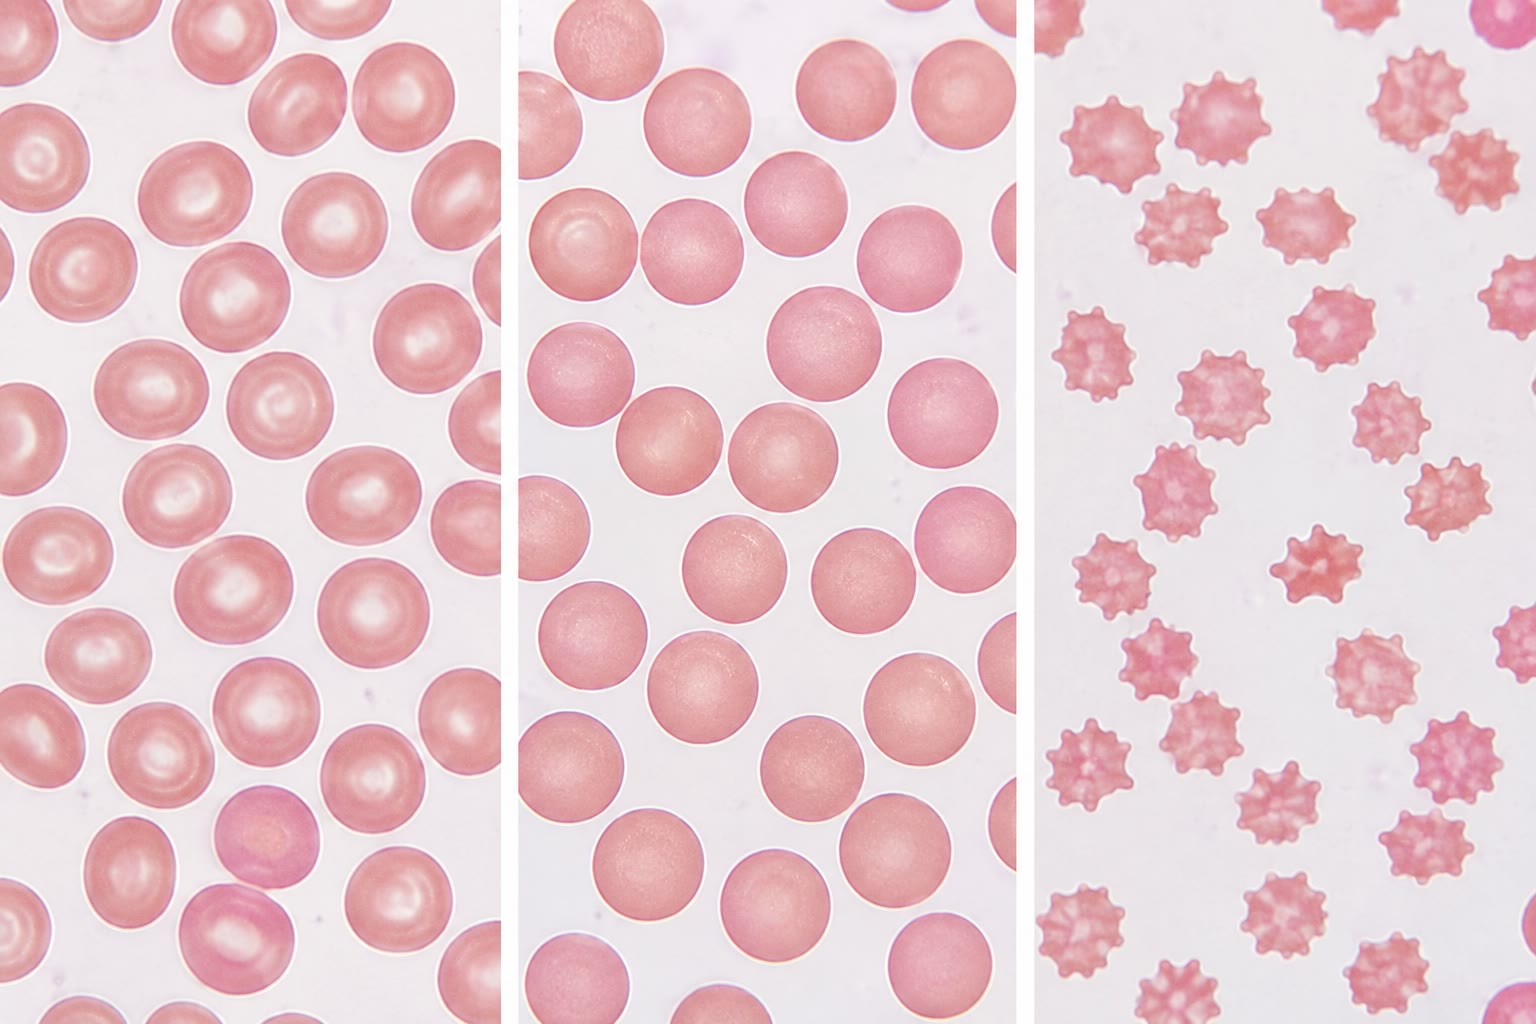
\includegraphics[width=0.78\linewidth]{images/book3/ai/b3-07-red-cells-osmosis.jpg}

{\small \omterm{def:b1:membranes-transport:osmosis}{समपरासरी} विलयन में लाल रक्त \omterm{def:b1:cell-unit-of-life:cell}{कोशिकाएँ} (उभयावतल चक्रिकाएँ), किसी
\omterm{def:b1:membranes-transport:osmosis}{अल्पपरासरी} विलयन में (फूलकर गोले, फटने को तैयार) और किसी \omterm{def:b1:membranes-transport:osmosis}{अतिपरासरी} विलयन
में (सिकुड़ी और दंतुरित)। जल अपने विभव के पीछे चलता है; और \omterm{def:b1:cell-unit-of-life:cell}{कोशिका} के पास
प्रतिरोध करने को कोई भित्ति नहीं है।}
\end{omfigure}

\begin{omfigure}
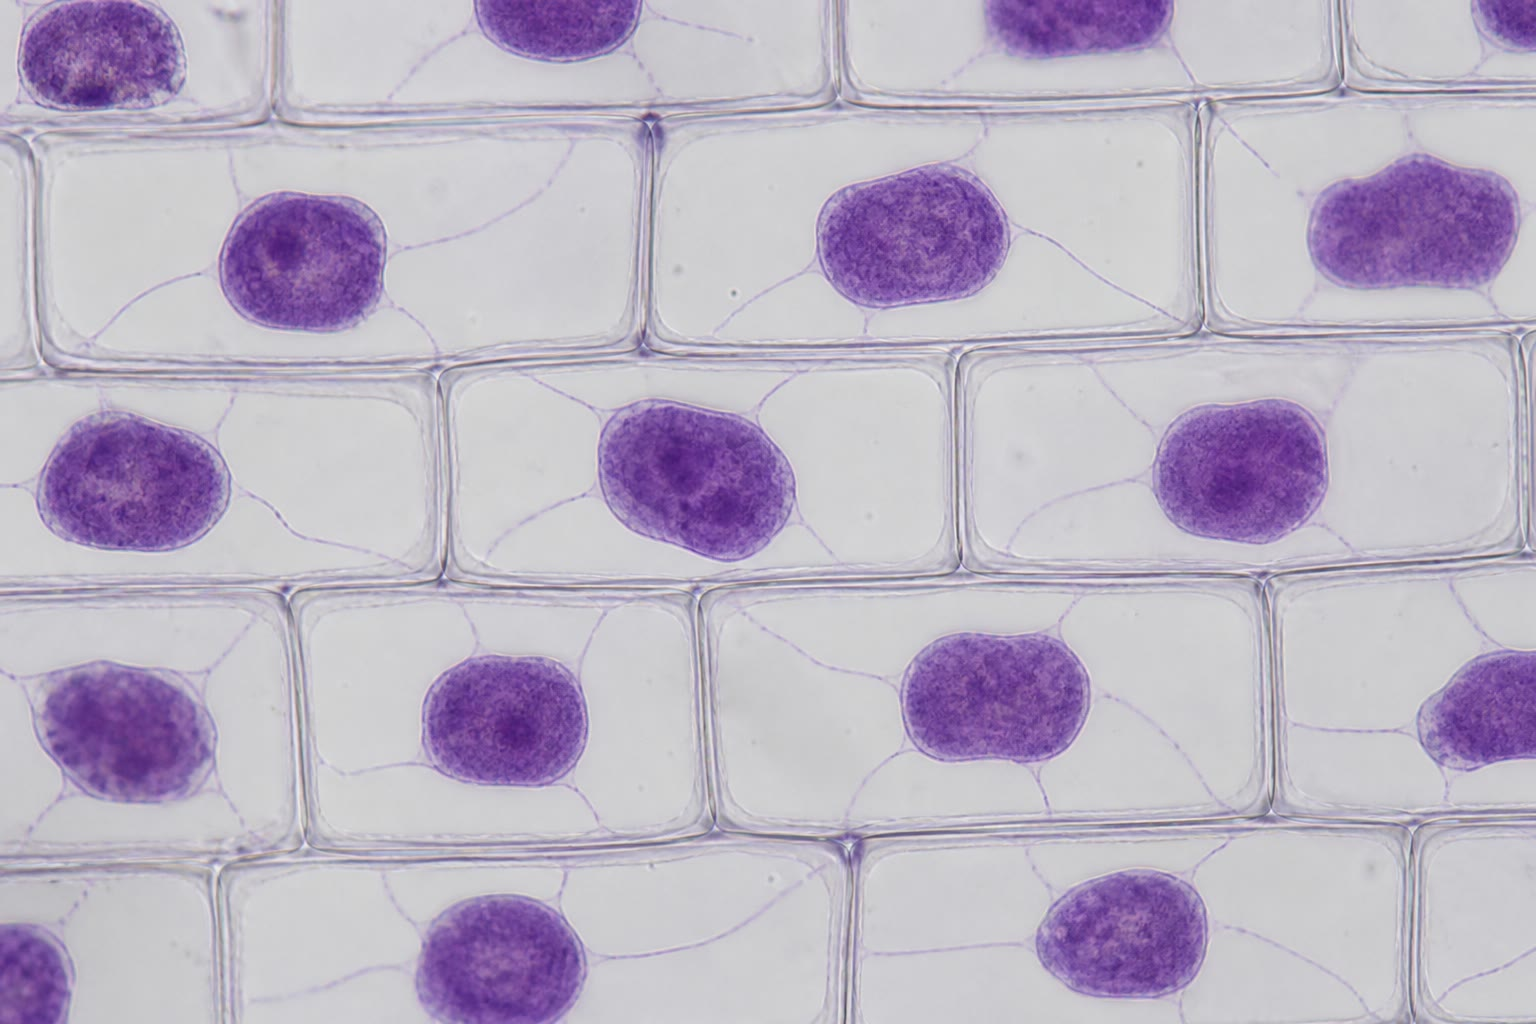
\includegraphics[width=0.6\linewidth]{images/book3/ai/b3-07-plasmolysis.jpg}

{\small जीवद्रव्यकुंचन: गाढ़े नमक के विलयन में प्याज़ की \omterm{def:b1:flowering-plant-organization:tissues}{अधिचर्म}। हर
\omterm{def:b1:cell-unit-of-life:cell}{कोशिका} का जीवद्रव्य जल खोकर कड़ी भित्ति से हट गया है, जो अपना रूप बनाए
रखती है। जल में जीवद्रव्य फिर फूलकर भित्ति से जा लगता और स्फीत होकर रुक
जाता।}
\end{omfigure}

\begin{example}[तीन विलयनों में एक लाल कोशिका]\label{ex:b1:membranes-transport:redcell}
प्लाज़्मा \qty{0.3}{osmol/L} है: दोनों ओर $\Psi_s = \qty{-0.74}{MPa}$,
इसलिए कोई शुद्ध प्रवाह नहीं। शुद्ध जल में ($\Psi = 0$) वह \omterm{def:b1:cell-unit-of-life:cell}{कोशिका}, जो
भीतर से \qty{-0.74}{MPa} पर है, तब तक जल लेती है जब तक उसकी झिल्ली, जो
केवल कुछ प्रतिशत ही खिंच सकती है, फट न जाए। \qty{0.6}{osmol/L} नमक में
वह तब तक जल खोती है जब तक उसका भीतर उतना ही सांद्र न हो जाए, यानी अपने
आधे आयतन पर। शुद्ध जल में कोई पादप \omterm{def:b1:cell-unit-of-life:cell}{कोशिका} नहीं फटती: जैसे-जैसे जल भीतर
आता है, भित्ति खिंचती है और $\Psi_p$ बढ़ता है, जब तक $\Psi_p = -\Psi_s$
न हो जाए, भीतर का \omterm{def:b1:membranes-transport:osmosis}{जल विभव} शून्य न हो जाए, और प्रवाह \qty{0.74}{MPa} पर
स्फीत \omterm{def:b1:cell-unit-of-life:cell}{कोशिका} के साथ रुक न जाए।
\end{example}

\begin{method}[जल-विभव का बहीखाता]\label{met:b1:membranes-transport:psi}
\begin{enumerate}
  \item हर विलेय-सांद्रता को ऑस्मोल में बदलिए (जो लवण दो आयनों में
        वियोजित होता है वह दो बार गिना जाता है) और $\Psi_s =
        -RTc_s$ निकालिए।
  \item दाब-पद जोड़िए: किसी खुले पात्र के विलयन या किसी जंतु \omterm{def:b1:cell-unit-of-life:cell}{कोशिका} के
        लिए $\Psi_p = 0$, किसी स्फीत पादप \omterm{def:b1:cell-unit-of-life:cell}{कोशिका} के लिए धनात्मक, और
        किसी \omterm{def:b1:flowering-plant-organization:tissues}{जाइलम} वाहिका में तनाव के नीचे के जल के लिए ऋणात्मक।
  \item जल नीचे वाले $\Psi$ की ओर बहता है। साम्य तब आता है जब दोनों
        $\Psi$ बराबर हो जाएँ: \omterm{def:b1:cell-unit-of-life:cell}{कोशिका} की अंतर्वस्तु के तनुकरण से (जंतु
        \omterm{def:b1:cell-unit-of-life:cell}{कोशिका}), या दाब के बढ़ने से (पादप \omterm{def:b1:cell-unit-of-life:cell}{कोशिका})।
  \item परिणाम का चिह्न प्रवाह की दिशा के रूप में पढ़िए, और उसका
        परिमाण प्रेरक बल के रूप में; प्रवाह की दर झिल्ली की जल-पारगम्यता
        पर भी निर्भर है, जिसे \omterm{def:b1:membranes-transport:transporters}{जलद्वारिका} \omterm{def:b1:membranes-transport:transporters}{चैनल} सौ गुना बढ़ा देते हैं।
\end{enumerate}
\end{method}

\section{अभिगमन प्रोटीन}

\begin{definition}[चैनल, वाहक, पंप]\label{def:b1:membranes-transport:transporters}
\emph{चैनल}\index{चैनल} ऐसे \omterm{def:b1:membranes-transport:proteins}{अंतर्वेशी प्रोटीन} हैं जिनमें जल से भरा एक
छिद्र है, जिससे होकर कोई विशिष्ट आयन या छोटा अणु अपनी प्रवणता के नीचे
प्रति सेकंड $10^8$ तक की दर से विसरित होता है; अनेक चैनल
\emph{द्वारित} होते हैं और किसी वोल्टता, किसी बंधक या किसी यांत्रिक बल
की अनुक्रिया में खुलते हैं। \emph{जलद्वारिका}\index{जलद्वारिका} जल के
चैनल हैं। \emph{वाहक}\index{वाहक} अपने विलेय को एक फलक पर बाँधते हैं,
संरूपण बदलते हैं, और उसे दूसरे फलक पर छोड़ देते हैं, अधिक से अधिक प्रति
सेकंड एक हज़ार बार; लाल \omterm{def:b1:cell-unit-of-life:cell}{कोशिका} का ग्लूकोज़ अभिगमक ऐसा ही है। प्रवणता के
नीचे काम करते चैनल और वाहक \emph{सुसाध्य
विसरण}\index{सुसाध्य विसरण} करते हैं, जो निष्क्रिय है पर चयनात्मक और
संतृप्य भी। \emph{पंप}\index{पंप} वे वाहक हैं जो किसी विलेय के उसकी
प्रवणता के विरुद्ध अभिगमन को ATP के जल-अपघटन से युग्मित करते हैं: यही
\emph{प्राथमिक सक्रिय अभिगमन}\index{सक्रिय अभिगमन} है। जंतु \omterm{def:b1:cell-unit-of-life:cell}{कोशिकाओं} का
\emph{सोडियम--पोटैशियम पंप}\index{सोडियम--पोटैशियम पंप} प्रति ATP तीन
$\mathrm{Na^+}$ बाहर और दो $\mathrm{K^+}$ भीतर ले जाता है; और पादप, कवक
तथा जीवाणु झिल्लियों का \emph{प्रोटॉन पंप} $\mathrm{H^+}$ बाहर ले जाता
है।
\end{definition}

\begin{omfigure}
\begin{tikzpicture}[font=\footnotesize, >=Stealth, line cap=round]
  % membrane band
  \fill[omDef!15] (0,0) rectangle (13.1,1.2);
  \draw[omDef!60!black] (0,0) -- (13.1,0) (0,1.2) -- (13.1,1.2);
  \node[anchor=east, gray, align=right] at (-0.15,1.5) {बाहर\\ (उच्च $\mathrm{Na^+}$, निम्न $\mathrm{K^+}$)};
  \node[anchor=east, gray, align=right] at (-0.15,-0.3) {कोशिकाद्रव\\ (निम्न $\mathrm{Na^+}$, उच्च $\mathrm{K^+}$)};
  % simple diffusion
  \draw[->, thick, omProp] (1.0,2.0) -- (1.0,-0.8);
  \node[anchor=south, align=center] at (1.0,2.1) {सरल विसरण\\ $\mathrm{O_2}$, $\mathrm{CO_2}$};
  % channel
  \draw[thick, omThm!80!black, fill=omThm!30, rounded corners=2pt] (2.6,-0.2) rectangle (3.0,1.4);
  \draw[thick, omThm!80!black, fill=omThm!30, rounded corners=2pt] (3.3,-0.2) rectangle (3.7,1.4);
  \draw[->, thick, omProp] (3.15,2.0) -- (3.15,-0.8);
  \node[anchor=south, align=center] at (3.15,2.1) {चैनल\\ $\mathrm{K^+}$, जल};
  % carrier (facilitated)
  \draw[thick, omThm!80!black, fill=omThm!30, rounded corners=5pt] (5.0,-0.3) rectangle (6.0,1.5);
  \draw[->, thick, omProp] (5.5,2.0) -- (5.5,1.55);
  \draw[->, thick, omProp] (5.5,-0.35) -- (5.5,-0.8);
  \node[anchor=south, align=center] at (5.5,2.1) {वाहक\\ ग्लूकोज़};
  \node[align=center, font=\scriptsize] at (5.5,0.6) {बाँधता है,\\ पलटता है};
  % pump
  \draw[thick, omExo!80!black, fill=omExo!30, rounded corners=5pt] (7.5,-0.3) rectangle (8.7,1.5);
  \draw[->, very thick, omExo!80!black] (7.8,-0.8) -- (7.8,2.0);
  \draw[->, very thick, omExo!80!black] (8.4,2.0) -- (8.4,-0.8);
  \node[anchor=south, align=center] at (8.1,2.1) {पंप\\ $3\,\mathrm{Na^+}$ बाहर, $2\,\mathrm{K^+}$ भीतर};
  \node[anchor=north, align=center, font=\scriptsize] at (8.1,-0.85) {ATP $\to$ ADP};
  % secondary active (symport)
  \draw[thick, omThm!80!black, fill=omThm!30, rounded corners=5pt] (11.0,-0.3) rectangle (12.2,1.5);
  \draw[->, very thick, omProp] (11.3,2.0) -- (11.3,-0.8);
  \draw[->, very thick, omExo!80!black] (11.9,2.0) -- (11.9,-0.8);
  \node[anchor=south, align=center] at (11.6,2.1) {सहवहन\\ $\mathrm{Na^+}$ नीचे, ग्लूकोज़ ऊपर};
  \node[anchor=north, align=center, font=\scriptsize] at (11.6,-0.85) {द्वितीयक सक्रिय};
  \node[anchor=north west, align=left, gray, font=\scriptsize] at (0,-1.5) {नारंगी तीर: प्रवणता के नीचे (निष्क्रिय); हरा: उसके विरुद्ध (सक्रिय)};
\end{tikzpicture}

{\small पार जाने के पाँच ढंग। लिपिड से होकर सरल विसरण; एक \omterm{def:b1:membranes-transport:transporters}{चैनल} और एक
वाहक (\omterm{def:b1:membranes-transport:transporters}{सुसाध्य विसरण}, प्रवणता के नीचे); \omterm{def:b1:membranes-transport:transporters}{सोडियम--पोटैशियम पंप} (\omterm{def:b1:membranes-transport:transporters}{प्राथमिक
सक्रिय अभिगमन}, ATP में चुकाया गया); और एक \omterm{prop:b1:membranes-transport:secondary}{सहवाहक} जो पंप की बनाई सोडियम
प्रवणता से ग्लूकोज़ को ऊपर की ओर घसीटता है (\omterm{prop:b1:membranes-transport:secondary}{द्वितीयक सक्रिय अभिगमन})।}
\end{omfigure}

\begin{proposition}[द्वितीयक सक्रिय अभिगमन]\label{prop:b1:membranes-transport:secondary}
\index{द्वितीयक सक्रिय अभिगमन}
किसी पंप की बनाई प्रवणता ऊर्जा का वह भंडार है जिसे दूसरे वाहक ख़र्च करते
हैं: कोई \emph{सहवाहक}\index{सहवाहक} किसी विलेय को उसी दिशा में नीचे
जाते किसी आयन से युग्मित करके ऊपर ले जाता है (आँत और गुर्दे का
सोडियम--ग्लूकोज़ अभिगमक; फ्लोएम का प्रोटॉन--सुक्रोस अभिगमक), जबकि कोई
\emph{प्रतिवाहक}\index{प्रतिवाहक} उसे विपरीत दिशा में जाते किसी आयन से
युग्मित करता है (सोडियम--कैल्सियम विनिमयक)। जंतु \omterm{def:b1:cell-unit-of-life:cell}{कोशिकाओं} में मुद्रा
$\mathrm{Na^+}$ प्रवणता है; और पौधों, कवकों तथा जीवाणुओं में
$\mathrm{H^+}$ प्रवणता।
\end{proposition}

\begin{example}[बलगतिकी क्रियाविधि बता देती है]\label{ex:b1:membranes-transport:kinetics}
किसी लाल \omterm{def:b1:cell-unit-of-life:cell}{कोशिका} में ग्लूकोज़ का फ्लक्स बाहरी सांद्रता के साथ बढ़ता है,
फिर किसी एंजाइम की तरह किसी अधिकतम पर सपाट हो जाता है
(\cref{ch:b1:enzymes}): यानी कोई वाहक, संतृप्य, जिसका $K_m$ लगभग
\qty{1.5}{mmol/L} है; और उससे मिलती-जुलती शर्करा, मैनोस, उसके लिए
स्पर्धा करती है। यूरिया का फ्लक्स उसकी सांद्रता के समानुपात में बिना
किसी सीमा के बढ़ता है: यानी सरल विसरण। आँत की किसी \omterm{def:b1:cell-unit-of-life:cell}{कोशिका} में ग्लूकोज़
का फ्लक्स तब रुक जाता है जब अवकाशिका से सोडियम हटा दिया जाए, या जब पंप
को ऊऐबेन से विषाक्त कर दिया जाए: यानी \omterm{prop:b1:membranes-transport:secondary}{द्वितीयक सक्रिय अभिगमन}।
\end{example}

\section{झिल्ली विभव}

\begin{definition}[झिल्ली विभव]\label{def:b1:membranes-transport:potential}
हर जीवित \omterm{def:b1:cell-unit-of-life:cell}{कोशिका} अपनी \omterm{def:b1:membranes-transport:membrane}{प्लाज़्मा झिल्ली} के आरपार एक विद्युत विभवांतर रखती
है, यानी \emph{झिल्ली विभव}\index{झिल्ली विभव} $V_m = V_{\text{भीतर}} - V_{\text{बाहर}}$, जो भीतर से ऋणात्मक है:
किसी \omterm{def:b1:body-plans-tissues:nervous}{न्यूरॉन} में \qty{-70}{mV}, किसी पेशी तंतु में \qty{-90}{mV}, और
किसी पादप \omterm{def:b1:cell-unit-of-life:cell}{कोशिका} में \qty{-120}{mV} या उससे भी अधिक। वह इसलिए उठता है कि
झिल्ली उन आयनों के लिए चयनात्मक रूप से पारगम्य है जिनकी सांद्रताएँ उसके
आरपार भिन्न हैं।
\end{definition}

\begin{theorem}[नर्न्स्ट समीकरण]\label{thm:b1:membranes-transport:nernst}
\index{नर्न्स्ट समीकरण}\index{साम्य विभव}
$z$ आवेश का कोई आयन, जिसकी सांद्रताएँ $c_{\text{बाहर}}$ और
$c_{\text{भीतर}}$ हैं, झिल्ली के आरपार साम्य में तब है --- यानी कोई
शुद्ध फ्लक्स नहीं, यद्यपि झिल्ली उसके लिए पारगम्य है --- जब विभव उसके
\emph{\omterm{thm:b1:membranes-transport:nernst}{साम्य विभव}} के बराबर हो
\[
E_{\text{आयन}} = \frac{RT}{zF}\,\ln\frac{c_{\text{बाहर}}}{c_{\text{भीतर}}}
= \frac{\qty{61.5}{mV}}{z}\,\log_{10}\frac{c_{\text{बाहर}}}{c_{\text{भीतर}}}
\quad (\qty{37}{\celsius}).
\]
\qty{5}{mmol/L} बाहर और \qty{140}{mmol/L} भीतर वाले $\mathrm{K^+}$ के
लिए $E_K = 61.5\log(5/140) = \qty{-89}{mV}$; और \qty{145}{} बाहर तथा
\qty{12}{} भीतर वाले $\mathrm{Na^+}$ के लिए $E_{Na} = \qty{+67}{mV}$।
\end{theorem}
\begin{proof}
उस आयन का एक मोल बाहर से भीतर ले जाने पर मुक्त ऊर्जा एक सांद्रता-पद और
एक विद्युत पद के योग से बदलती है:
\[
\Delta G = RT\ln\frac{c_{\text{भीतर}}}{c_{\text{बाहर}}} + zFV_m .
\]
साम्य पर $\Delta G = 0$, जिससे $V_m = (RT/zF)\ln(c_{\text{बाहर}}/c_{\text{भीतर}})$ मिलता है।
दस-आधार लघुगणकों में बदलने और $R = \qty{8.314}{J.mol^{-1}.K^{-1}}$,
$T = \qty{310}{K}$, $F = \qty{96485}{C/mol}$ रखने पर संख्यात्मक रूप मिल
जाता है।
\end{proof}

\begin{proposition}[विश्राम विभव का उद्गम]\label{prop:b1:membranes-transport:resting}
विश्राम में झिल्ली $\mathrm{K^+}$ के लिए (खुले पोटैशियम \omterm{def:b1:membranes-transport:transporters}{चैनलों} से होकर)
$\mathrm{Na^+}$ की तुलना में कहीं अधिक पारगम्य है; $\mathrm{K^+}$ अपनी
सांद्रता-प्रवणता के नीचे रिसकर बाहर जाता है और भीतर को ऋणात्मक छोड़
जाता है, जब तक पीछे खींचता विद्युत बल उस रिसाव को लगभग संतुलित न कर दे।
इसलिए विश्राम विभव $E_K$ के पास रहता है, और छोटे सोडियम रिसाव से
$E_{Na}$ की ओर थोड़ा खिंच जाता है (गोल्डमैन समीकरण हर आयन के नर्न्स्ट पद
को उसकी पारगम्यता से तोलता है)। पंप उन प्रवणताओं को बनाए रखता है जिन्हें
रिसाव अन्यथा क्षय कर देते; वह कुछ मिलीवोल्ट सीधे भी जोड़ता है, क्योंकि
वह दो आवेश भीतर लाने के बदले तीन बाहर ले जाता है।
\end{proposition}
\begin{proof}[साक्ष्य]
किसी स्क्विड अक्षतंतु में, जब बाहरी पोटैशियम एक विस्तृत परास में बदला
जाता है, तो विश्राम विभव $E_K$ के पीछे चलता है (उच्च सांद्रताओं पर प्रति
दशक \qty{58}{mV} प्रवणता की एक सरल रेखा), और निम्न सांद्रताओं पर उससे
ठीक उसी तरह हटता है जैसी भविष्यवाणी कोई छोटी सोडियम पारगम्यता करती है।
पंप को ऊऐबेन से रोक देने पर विभव मिनटों तक लगभग अपरिवर्तित रहता है, फिर
घंटों में क्षय होता जाता है जैसे-जैसे प्रवणताएँ चुकती हैं: विभव एक
विसरण विभव है, और पंप उसका दीर्घकालिक सहारा।
\end{proof}

\begin{omfigure}
\begin{tikzpicture}
\begin{semilogxaxis}[
  width=0.86\linewidth, height=6.2cm,
  axis x line=bottom, axis y line=left,
  xmin=0.8, xmax=200, ymin=-135, ymax=10,
  xlabel={बाहरी $\mathrm{K^+}$ (\unit{mmol/L})}, ylabel={झिल्ली विभव (\unit{mV})},
  xlabel style={font=\small, at={(axis description cs:0.5,-0.12)}, anchor=north},
  ylabel style={font=\small},
  tick label style={font=\small}, xtick={1,10,100}, log ticks with fixed point, ytick={-120,-100,-80,-60,-40,-20,0},
  legend style={font=\small, at={(0.03,0.97)}, anchor=north west, draw=none},
  clip=false,
]
\addplot[thick, dashed, omDef, domain=0.8:200, samples=40] {58*log10(x/140)};
\addlegendentry{नर्न्स्ट $E_K$ (प्रति दशक \qty{58}{mV} प्रवणता)}
\addplot[very thick, omThm, domain=0.8:200, samples=60] {58*log10((x+0.01*145)/(140+0.01*12))};
\addlegendentry{मापा गया: $\mathrm{K^+}$ और एक छोटा $\mathrm{Na^+}$ रिसाव}
\draw[dashed, gray] (axis cs:5,-135) -- (axis cs:5,-82);
\node[font=\scriptsize, anchor=west] at (axis cs:5.5,-120) {शरीरक्रियात्मक \qty{5}{mmol/L}};
\end{semilogxaxis}
\end{tikzpicture}

{\small बाहरी पोटैशियम के सापेक्ष विश्राम विभव। उच्च पोटैशियम पर झिल्ली
किसी पोटैशियम इलेक्ट्रोड की तरह व्यवहार करती है और नर्न्स्ट रेखा के पीछे
चलती है; निम्न पोटैशियम पर छोटा सोडियम रिसाव उसे $E_K$ से ऊपर खींच लेता
है।}
\end{omfigure}

\begin{example}[पंप की ऊर्जा कहाँ जाती है]\label{ex:b1:membranes-transport:pumpcost}
एक $\mathrm{Na^+}$ को \qty{12}{} से \qty{145}{mmol/L} के विरुद्ध और
\qty{-70}{mV} के विरुद्ध बाहर पंप करने में $RT\ln(145/12) + F\times 0.070 = 6.4 + 6.8 =
\qty{13.2}{kJ/mol}$ लगते हैं; तीन के लिए \qty{40}{kJ}, और साथ में दो
$\mathrm{K^+}$ भीतर लाने पर प्रति आयन $RT\ln(140/5) - F\times 0.070 = 8.6 - 6.8 =
\qty{1.8}{kJ/mol}$: यानी प्रति चक्र \qty{43}{kJ}, जबकि कोशिकीय
परिस्थितियों में एक ATP \qty{50}{kJ} देता है। पंप अपनी ऊष्मागतिक सीमा के
पास चलता है, और वह विश्राम कर रहे किसी जंतु के ATP का एक-तिहाई ख़र्च
करता है, मस्तिष्क में दो-तिहाई।
\end{example}

\section{थोक अभिगमन}

\begin{proposition}[पुटिकीय अभिगमन]\label{prop:b1:membranes-transport:vesicles}
वृहदणु और कण \omterm{def:b1:membranes-transport:membrane}{प्लाज़्मा झिल्ली} से होकर गुज़रे बिना ही उसे पार करते हैं:
\emph{बहिर्क्षेपण} में कोई पुटिका झिल्ली से जुड़कर बाहर की ओर ख़ाली हो
जाती है; \emph{\omterm{def:b1:eukaryotic-cell:endocytosis}{अंतर्ग्रहण}} में झिल्ली सामग्री को किसी पुटिका में निगल
लेती है (\cref{ch:b1:eukaryotic-cell})। दोनों को ATP चाहिए, दोनों
अंतर्वस्तु के साथ-साथ झिल्ली भी चलाते हैं, और दोनों झिल्ली का पक्षभेद
बनाए रखते हैं। झिल्ली पार करने के तीनों मार्ग --- लिपिड से होकर, किसी
प्रोटीन से होकर, किसी पुटिका के भीतर --- तीन तरह से चयनात्मक हैं:
विलेयता से, आणविक अभिज्ञान से, और इस चुनाव से कि निगला क्या जाए।
\end{proposition}

\begin{example}[कोलेस्टेरॉल की आपूर्ति]\label{ex:b1:membranes-transport:ldl}
कोलेस्टेरॉल रक्त में प्रोटीन से लिपे उन कणों के भीतर चलता है जो किसी भी
वाहक के लिए बहुत बड़े हैं। जिस \omterm{def:b1:cell-unit-of-life:cell}{कोशिका} को कोलेस्टेरॉल चाहिए वह उस कण के
लिए ग्राही प्रदर्शित करती है; कण और ग्राही किसी लिपे गड्ढे में इकट्ठे
होते हैं, जो चुटककर अलग हो जाता है, और वह पुटिका उस कण को किसी \omterm{def:b1:eukaryotic-cell:endomembrane}{लयनकाय}
तक पहुँचा देती है जहाँ कोलेस्टेरॉल मुक्त होता है। जिस व्यक्ति के ग्राही
दोषपूर्ण हों वह उन कणों को हटा नहीं पाता: रक्त का कोलेस्टेरॉल दुगुना हो
जाता है और वयस्कता के आरंभ में ही धमनियाँ जाम हो जाती हैं। एक \omterm{def:b1:membranes-transport:membrane}{झिल्ली
प्रोटीन}, एक रोग।
\end{example}

\section{अभ्यास}

\begin{exercise}[$\star$]\label{exo:b1:membranes-transport:1}
\omterm{def:b1:membranes-transport:membrane}{तरल मोज़ेक मॉडल} का चार वाक्यों में वर्णन कीजिए: लिपिड, प्रोटीन, तरलता,
असममिति।
\end{exercise}

\begin{exercise}[$\star$]\label{exo:b1:membranes-transport:2}
$\mathrm{O_2}$, ग्लूकोज़, $\mathrm{Na^+}$, जल और एथेनॉल को किसी शुद्ध
\omterm{def:b1:membranes-transport:membrane}{लिपिड द्विस्तर} से होकर उनकी पारगम्यता के क्रम में रखिए, और क्रम समझाइए।
\end{exercise}

\begin{exercise}[$\star$]\label{exo:b1:membranes-transport:3}
\qty{25}{\celsius} पर \qty{0.1}{mol/L} सुक्रोस विलयन का और
\qty{0.1}{mol/L} NaCl विलयन का \omterm{def:b1:membranes-transport:osmosis}{विलेय विभव} निकालिए।
\end{exercise}

\begin{exercise}[$\star$]\label{exo:b1:membranes-transport:4}
\qty{37}{\celsius} पर \qty{120}{mmol/L} बाहर और \qty{4}{mmol/L} भीतर
वाले $\mathrm{Cl^-}$ का नर्न्स्ट विभव निकालिए। क्या \qty{-89}{mV} पर की
किसी \omterm{def:b1:cell-unit-of-life:cell}{कोशिका} में क्लोराइड साम्य में है?
\end{exercise}

\begin{exercise}[$\star\star$]\label{exo:b1:membranes-transport:5}
गॉर्टर और ग्रेंडल ने प्रति \omterm{def:b1:cell-unit-of-life:cell}{कोशिका} \qty{100}{\micro m^2} सतह वाली
$\num{4.7e9}$ लाल \omterm{def:b1:cell-unit-of-life:cell}{कोशिकाएँ} लीं और \qty{0.92}{m^2} की एकल लिपिड परत पाई।
एकल परत के क्षेत्रफल का कोशिका-सतह से अनुपात निकालिए और निष्कर्ष
दीजिए।
\end{exercise}

\begin{exercise}[$\star\star$]\label{exo:b1:membranes-transport:6}
किसी पादप \omterm{def:b1:cell-unit-of-life:cell}{कोशिका} का \omterm{def:b1:membranes-transport:osmosis}{विलेय विभव} \qty{-0.9}{MPa} और \omterm{def:b1:membranes-transport:osmosis}{दाब विभव}
\qty{0.5}{MPa} है। उसे किसी खुली तश्तरी में \qty{-0.6}{MPa} \omterm{def:b1:membranes-transport:osmosis}{विलेय विभव}
के विलयन में रखा जाता है। जल किस ओर चलेगा, और साम्य पर \omterm{def:b1:cell-unit-of-life:cell}{कोशिका} का \omterm{def:b1:membranes-transport:osmosis}{दाब
विभव} क्या होगा (मानिए कि उसका \omterm{def:b1:membranes-transport:osmosis}{विलेय विभव} नहीं बदलता)?
\end{exercise}

\begin{exercise}[$\star\star$]\label{exo:b1:membranes-transport:7}
किसी \omterm{def:b1:cell-unit-of-life:cell}{कोशिका} द्वारा ग्लूकोज़ का ग्रहण बढ़ती बाहरी सांद्रताओं पर मापा
जाता है: \qtylist{1;2;5;10;20}{mmol/L} पर
\qtylist{0.4;0.67;1.0;1.25;1.43}{\micro mol/min} मिलते हैं। दिखाइए कि
ग्रहण संतृप्त होता है, अधिकतम दर और उसकी आधी देने वाली सांद्रता आँकिए,
और क्रियाविधि का नाम बताइए।
\end{exercise}

\begin{exercise}[$\star\star$]\label{exo:b1:membranes-transport:8}
समझाइए कि किसी \omterm{def:b1:cell-unit-of-life:cell}{कोशिका} का विश्राम विभव $E_K$ के पास क्यों रहता है,
$E_{Na}$ के नहीं, और यदि सोडियम \omterm{def:b1:membranes-transport:transporters}{चैनल} अचानक खुल जाएँ तो उसका क्या होगा।
\end{exercise}

\begin{exercise}[$\star\star$]\label{exo:b1:membranes-transport:9}
सोडियम--ग्लूकोज़ \omterm{prop:b1:membranes-transport:secondary}{सहवाहक} प्रति ग्लूकोज़ दो $\mathrm{Na^+}$ ढोता है।
\qty{145}{mmol/L} बाहर और \qty{12}{} भीतर वाले $\mathrm{Na^+}$ के साथ
तथा $V_m = \qty{-60}{mV}$ के साथ, दोनों सोडियम आयनों से उपलब्ध मुक्त
ऊर्जा निकालिए और \qty{37}{\celsius} पर वह अधिकतम ग्लूकोज़
सांद्रता-अनुपात (भीतर/बाहर) भी जो \omterm{prop:b1:membranes-transport:secondary}{सहवाहक} बना सकता है।
\end{exercise}

\begin{exercise}[$\star\star\star$]\label{exo:b1:membranes-transport:10}
किसी \omterm{def:b1:cell-unit-of-life:cell}{कोशिका} को \qty{4}{\celsius} तक ठंडा किया जाता है। कारण सहित इन पर
पड़ते प्रभावों की भविष्यवाणी कीजिए: झिल्ली की तरलता, $\mathrm{O_2}$ का
सरल विसरण, पंप, घंटों में आयन-प्रवणताएँ, \omterm{def:b1:membranes-transport:potential}{झिल्ली विभव}, और \omterm{def:b1:cell-unit-of-life:cell}{कोशिका} का
आयतन। (ध्यान रखिए कि \omterm{def:b1:cell-unit-of-life:cell}{कोशिका} के प्रोटीन एक \omterm{def:b1:membranes-transport:osmosis}{परासरणी} खिंचाव लगाते हैं जिसे
सोडियम प्रवणता सामान्यतः संतुलित रखती है।)
\end{exercise}

\begin{exercise}[$\star\star\star$]\label{exo:b1:membranes-transport:11}
फ़्राई और एडिडिन की जुड़ी हुई \omterm{def:b1:cell-unit-of-life:cell}{कोशिकाओं} में सतही प्रोटीनों का पूरा मिश्रण
\qty{37}{\celsius} पर \qty{40}{min} में दिखा, \qty{4}{\celsius} पर कुछ
नहीं, और \qty{37}{\celsius} पर भी कुछ नहीं जब ATP संश्लेषण रोक दिया गया
--- बाद में यह अंतिम परिणाम ग़लत निकला। बताइए कि हर परिणाम मिश्रण की
क्रियाविधि के बारे में क्या दर्शाता, और सही रूप (मिश्रण को ATP नहीं
चाहिए) \omterm{def:b1:membranes-transport:membrane}{तरल मोज़ेक मॉडल} के लिए क्यों मायने रखता है।
\end{exercise}

\begin{exercise}[$\star\star\star$]\label{exo:b1:membranes-transport:12}
``\omterm{def:b1:membranes-transport:potential}{झिल्ली विभव} आयन-प्रवणताओं का उप-उत्पाद है, ऐसी कोई चीज़ नहीं जिसे
\omterm{def:b1:cell-unit-of-life:cell}{कोशिका} सीधे बनाती हो।'' \omterm{thm:b1:membranes-transport:nernst}{नर्न्स्ट समीकरण}, पंप, और झिल्ली को आवेशित करने
के लिए सचमुच जितने आयन चाहिए उनकी संख्या (धारिता
\qty{1}{\micro F/cm^2}) की सहायता से एक अनुच्छेद में चर्चा कीजिए।
\end{exercise}

\section{समस्या: आंत्रकोशिका}

\begin{problem}[{सप्ताहांत समस्या --- वह कोशिका जो आँत से ग्लूकोज़
खींच लेती है: पंप, सहवाहक, वाहक और नर्न्स्ट समीकरण, और अंत में वह
सर्वोच्च ग्लूकोज़ अनुपात जो कोशिका बना सकती है}]
\label{pb:b1:membranes-transport:1}
आँत की कोई \omterm{def:b1:body-plans-tissues:epithelium}{उपकला} \omterm{def:b1:cell-unit-of-life:cell}{कोशिका} (आंत्रकोशिका) \qty{25}{\micro m} ऊँची और
\qty{5}{\micro m} चौड़ी है; उसकी शीर्ष झिल्ली अवकाशिका की ओर है और
आधार-पार्श्व झिल्ली रक्त की ओर। उसके \omterm{def:b1:eukaryotic-cell:organelle}{कोशिकाद्रव} में \qty{12}{mmol/L}
$\mathrm{Na^+}$ और \qty{140}{mmol/L} $\mathrm{K^+}$ है; और अवकाशिका तथा
रक्त में \qty{145}{mmol/L} $\mathrm{Na^+}$ तथा \qty{5}{mmol/L}
$\mathrm{K^+}$। \omterm{def:b1:membranes-transport:potential}{झिल्ली विभव} \qty{-60}{mV} है।
$T = \qty{310}{K}$, $R = \qty{8.314}{J.mol^{-1}.K^{-1}}$,
$F = \qty{96500}{C/mol}$, $RT/F = \qty{26.7}{mV}$, और \omterm{def:b1:cell-unit-of-life:cell}{कोशिका} में
$\Delta G_{\text{ATP}} = \qty{-50}{kJ/mol}$ लीजिए।

\medskip
\noindent\textbf{भाग I --- प्रवणताएँ।}
\begin{enumerate}
  \item $\mathrm{Na^+}$ और $\mathrm{K^+}$ के नर्न्स्ट विभव निकालिए।
  \item \qty{-60}{mV} पर कौन-सा आयन साम्य के अधिक पास है? इससे विश्राम
        की पारगम्यताओं के बारे में क्या पता चलता है?
  \item \omterm{def:b1:cell-unit-of-life:cell}{कोशिका} में घुसते $\mathrm{Na^+}$ के एक मोल के लिए, और बाहर
        जाते $\mathrm{K^+}$ के एक मोल के लिए, मुक्त ऊर्जा का परिवर्तन
        निकालिए।
  \item पंप के एक चक्र ($3\,\mathrm{Na^+}$ बाहर, $2\,\mathrm{K^+}$
        भीतर) की मुक्त-ऊर्जा लागत निकालिए और उसकी तुलना एक ATP की ऊर्जा
        से कीजिए। दक्षता क्या है?
  \item पंप केवल आधार-पार्श्व झिल्ली पर है। समझाइए कि \omterm{def:b1:cell-unit-of-life:cell}{कोशिका} को
        ग्लूकोज़ अवकाशिका से रक्त तक ले जाने के लिए यह स्थान क्यों
        ज़रूरी है।
\end{enumerate}

\medskip
\noindent\textbf{भाग II --- ग्लूकोज़ ऊपर की ओर।}
शीर्ष झिल्ली पर ऐसा \omterm{prop:b1:membranes-transport:secondary}{सहवाहक} है जो एक ग्लूकोज़ के साथ दो $\mathrm{Na^+}$
भीतर लेता है; और आधार-पार्श्व झिल्ली पर कोई ग्लूकोज़ वाहक है (\omterm{def:b1:membranes-transport:transporters}{सुसाध्य
विसरण})।
\begin{enumerate}[resume]
  \item \omterm{def:b1:cell-unit-of-life:cell}{कोशिका} में घुसते दो $\mathrm{Na^+}$ से मुक्त हुई ऊर्जा
        निकालिए।
  \item एक ग्लूकोज़ को अवकाशिका (सांद्रता $c_L$) से \omterm{def:b1:eukaryotic-cell:organelle}{कोशिकाद्रव} ($c_C$)
        तक ले जाने के लिए चाहिए मुक्त ऊर्जा लिखिए।
  \item \omterm{prop:b1:membranes-transport:secondary}{सहवाहक} की सीमा पर दोनों बराबर हैं। अधिकतम अनुपात $c_C/c_L$
        निकालिए।
  \item यदि अवशोषण के अंत में अवकाशिका का ग्लूकोज़ \qty{0.1}{mmol/L}
        तक गिर जाए, तो \omterm{prop:b1:membranes-transport:secondary}{सहवाहक} \omterm{def:b1:eukaryotic-cell:organelle}{कोशिकाद्रव} में कौन-सी सांद्रता फिर भी
        बनाए रख सकता है?
  \item रक्त का ग्लूकोज़ \qty{5}{mmol/L} है। समझाइए कि ग्लूकोज़ बिना
        किसी और ऊर्जा के \omterm{def:b1:cell-unit-of-life:cell}{कोशिका} से रक्त में कैसे निकलता है।
  \item \omterm{prop:b1:membranes-transport:secondary}{सहवाहक} शीर्ष झिल्ली पर और वाहक आधार-पार्श्व झिल्ली पर क्यों रखे
        गए हैं, उल्टा क्यों नहीं?
  \item हैज़े के लिए मुँह से दी जाने वाली पुनर्जलीकरण विलयनों में
        ग्लूकोज़ और नमक होते हैं। \omterm{prop:b1:membranes-transport:secondary}{सहवाहक} से समझाइए कि ग्लूकोज़ नमक को
        --- और जल को --- अवशोषित क्यों करा देता है।
\end{enumerate}

\medskip
\noindent\textbf{भाग III --- आवागमन की गिनती।}
\omterm{def:b1:cell-unit-of-life:cell}{कोशिका} प्रति सेकंड \qty{2e-15}{mol} ग्लूकोज़ अवशोषित करती है।
\begin{enumerate}[resume]
  \item \omterm{prop:b1:membranes-transport:secondary}{सहवाहकों} से होकर प्रति सेकंड घुसते $\mathrm{Na^+}$ की मात्रा
        निकालिए, और उसे बाहर करने के लिए प्रति सेकंड चाहिए पंप-चक्रों
        की संख्या भी।
  \item इस निर्यात पर प्रति सेकंड ख़र्च ATP निकालिए, और अवशोषित
        ग्लूकोज़ का वह भिन्न भी जिसे उसकी क़ीमत चुकाने के लिए श्वसन में
        जलाना पड़ेगा (प्रति ग्लूकोज़ लगभग 30 ATP)।
  \item हर \omterm{prop:b1:membranes-transport:secondary}{सहवाहक} प्रति सेकंड \qty{50}{} चक्र लगाता है। शीर्ष झिल्ली को
        कितने \omterm{prop:b1:membranes-transport:secondary}{सहवाहक} चाहिए? शीर्ष झिल्ली \qty{25}{\micro m^2} की है
        जिसे सूक्ष्मांकुर \qty{20}{} गुना कर देते हैं: प्रति वर्ग
        माइक्रोमीटर \omterm{prop:b1:membranes-transport:secondary}{सहवाहकों} का घनत्व निकालिए।
  \item जो $\mathrm{Na^+}$ भीतर आता है वह \omterm{def:b1:membranes-transport:osmosis}{परासरण} से जल भी लाता है। दो
        $\mathrm{Na^+}$ और एक ग्लूकोज़, साथ आते $\mathrm{Cl^-}$ सहित,
        चार ऑस्मोल हैं; और \omterm{def:b1:cell-unit-of-life:cell}{कोशिका} अपनी परासरणीयता \qty{0.3}{osmol/L} पर
        रखती है। वह जल-आयतन निकालिए जिसे प्रति सेकंड विलेयों के पीछे
        आना चाहिए, और वह समय भी जो \omterm{def:b1:cell-unit-of-life:cell}{कोशिका} का आयतन दुगुना करने में लगता
        यदि जल आधार-पार्श्व झिल्ली से बाहर न जाता।
  \item प्रति ग्लूकोज़ अणु अवशोषित जल अणुओं की संख्या निकालिए
        (\qty{18}{g/mol}, घनत्व \qty{1}{g/mL})।
\end{enumerate}

\medskip
\noindent\textbf{भाग IV --- झिल्ली को आवेशित करना।}
झिल्ली \qty{1}{\micro F/cm^2} का एक संधारित्र है।
\begin{enumerate}[resume]
  \item \omterm{def:b1:cell-unit-of-life:cell}{कोशिका} की झिल्ली का क्षेत्रफल (सूक्ष्मांकुरों के बिना
        \qty{25}{\micro m} गुणा \qty{5}{\micro m} गुणा
        \qty{5}{\micro m} का एक डिब्बा मानकर) और उसकी धारिता निकालिए।
  \item \qty{-60}{mV} बनाए रखने के लिए चाहिए आवेश और उसके बराबर एकसंयोजी
        आयनों की संख्या निकालिए।
  \item यह झिल्ली के प्रति वर्ग माइक्रोमीटर कितने अतिरिक्त आयनों के
        बराबर है, यह निकालिए।
  \item \omterm{def:b1:cell-unit-of-life:cell}{कोशिका} में $\mathrm{K^+}$ आयनों की संख्या निकालिए, और वह भिन्न
        भी जिसे झिल्ली आवेशित करने के लिए बाहर जाना पड़ता है। टिप्पणी
        कीजिए।
  \item पंप हर चक्र पर एक शुद्ध आवेश बाहर ले जाता है। प्रश्न 13 की
        सहायता से वह धारा निकालिए जो वह ढोता है, और वह विभव-परिवर्तन भी
        जो वह एक सेकंड में पैदा करता यदि और कुछ न चलता। विभव सचमुच
        बेक़ाबू क्यों नहीं होता?
  \item कोई दवा पंप को रोक देती है। क्रम से सोडियम प्रवणता, ग्लूकोज़
        अवशोषण, \omterm{def:b1:membranes-transport:potential}{झिल्ली विभव} और \omterm{def:b1:cell-unit-of-life:cell}{कोशिका} के आयतन में परिवर्तनों की
        भविष्यवाणी कीजिए।
  \item इसके बजाय कोई दवा पोटैशियम \omterm{def:b1:membranes-transport:transporters}{चैनल} रोक देती है। विश्राम विभव में
        परिवर्तन की भविष्यवाणी कीजिए।
  \item परिणाम बताइए: वह अधिकतम ग्लूकोज़ सांद्रता-अनुपात जो
        आंत्रकोशिका बना सकती है, और वे दो \omterm{def:b1:membranes-transport:membrane}{झिल्ली प्रोटीन} जो उसे संभव
        बनाते हैं।
\end{enumerate}
\end{problem}
